%% Stable but Not Correct — ACM Web Conference (TheWebConf) 2027 submission draft
%% Anonymous double-blind review version.
%% Build: pdflatex main && bibtex main && pdflatex main && pdflatex main
%% Camera-ready: remove [anonymous,review], add rights commands from the ACM
%% e-Rights form, restore author block.
\documentclass[sigconf,anonymous,review]{acmart}

\usepackage{booktabs}
\usepackage{amsmath}
\usepackage{graphicx}

%% Submission draft: ACM reference block and CCS render as they will in the
%% submitted PDF. Copyright strip is suppressed until the e-Rights form is
%% completed (ACM supplies the real commands at camera-ready).
\renewcommand\footnotetextcopyrightpermission[1]{}

\begin{document}

\title{Stable but Not Correct: Auditing Multi-Agent LLM Debate as a
Reliability Mechanism for High-Stakes Financial Information Access}

\author{Anonymous Author(s)}

\begin{abstract}
Web-facing assistants increasingly answer high-stakes financial questions,
and multi-agent LLM debate---having several model instances argue before
answering---is being adopted as a reliability mechanism for exactly such
systems. We audit whether it delivers. Using 139 expert-labelled questions
over public company filings and market indicators, four open-weights models,
and a second benchmark for external validity, we find that debate makes
answers markedly \emph{more stable} without making them \emph{more correct}.
The reason is a failure mode that accuracy metrics and standard uncertainty
instrumentation both obscure: these systems express uncertainty
\emph{categorically}, converging with near-zero entropy on non-committal
answers (``it depends'', ``insufficient data'') rather than spreading
probability across alternatives. We introduce non-commitment mass,
$p_{\mathrm{nc}}$, alongside an exact aleatoric/epistemic entropy
decomposition, and characterise three user-facing failure modes:
\emph{hedge collision}, where the system declines to answer a question the
reference answer settles ($44.3$--$66.3\%$ of all errors); \emph{wrong-direction
commitment}, confident but incorrect entity selection, which dominates
screening-style queries (up to $77\%$ of their errors) and is invisible to every
uncertainty channel we measure; and \emph{overcommitment} on questions whose
correct answer is genuinely a refusal. Which mode a system exhibits is a
property of the model \emph{and} the query type, not of model scale: the
cross-signal query lane is the highest-hedging lane in all five systems
tested. Controlled interventions show the uncertainty channels are not
evidence-responsive---injecting contradictory evidence \emph{lowers} measured
disagreement as both agents retreat to a shared hedge---and matched
agent-design controls show that a single biased participant, not debate
itself, drives catastrophic degradation. For operators of high-stakes
information services, the practical consequence is that debate should be
treated as a stability mechanism whose failures are categorical, monitored
by non-commitment rate rather than by entropy.
\end{abstract}

\begin{CCSXML}
<ccs2012>
<concept><concept_id>10002951.10003317</concept_id>
<concept_desc>Information systems~Information retrieval</concept_desc>
<concept_significance>500</concept_significance></concept>
<concept><concept_id>10010147.10010178.10010187</concept_id>
<concept_desc>Computing methodologies~Multi-agent systems</concept_desc>
<concept_significance>500</concept_significance></concept>
<concept><concept_id>10010147.10010178.10010179</concept_id>
<concept_desc>Computing methodologies~Natural language processing</concept_desc>
<concept_significance>300</concept_significance></concept>
<concept><concept_id>10003456.10003462</concept_id>
<concept_desc>Social and professional topics~Computing / technology policy</concept_desc>
<concept_significance>300</concept_significance></concept>
</ccs2012>
\end{CCSXML}

\ccsdesc[500]{Information systems~Information retrieval}
\ccsdesc[500]{Computing methodologies~Multi-agent systems}
\ccsdesc[300]{Computing methodologies~Natural language processing}
\ccsdesc[300]{Social and professional topics~Computing / technology policy}

\keywords{multi-agent debate, large language models, uncertainty
quantification, responsible AI, financial information access, evaluation}

\maketitle

\section{Introduction}

Financial question answering has moved onto the open web. Retail investors,
journalists and analysts increasingly put questions about company health,
valuation and market signals to LLM-backed assistants rather than to
databases or human advisers, and the answers they receive influence
consequential decisions. This is a high-stakes information-access setting in
the classic sense: the cost of a confidently wrong answer is borne by the
user, the provenance of the answer is opaque, and the failure is often
invisible at the point of consumption.

The dominant proposed remedy is architectural. Rather than trusting one
model, deployed systems increasingly run \emph{multi-agent debate}: several
model instances answer independently, exchange arguments, and converge on a
response~\cite{du2023debate}. Debate is attractive to operators precisely
because it looks like a reliability mechanism---disagreement gets surfaced
and resolved before the user sees anything. A parallel line of work supplies
the instrumentation: treat the system as a distribution over answers and
measure its entropy, decomposed into reducible (epistemic) and irreducible
(aleatoric) parts~\cite{kuhn2023semantic,depeweg2018decomposition}.

This paper audits that pairing. We ask a deployment question---\emph{does
debate make a web-facing financial assistant more reliable, and would the
standard instrumentation tell us if it did not?}---and answer both parts in
the negative, for reasons that turn out to be structural rather than
incidental.

\paragraph{Debate buys stability, not correctness.} Across four open-weights
models on 139 expert-labelled questions, one debate round reliably reduces
within-agent instability (up to $-0.149$ normalised, $p < 10^{-6}$) while
leaving between-agent disagreement flat and leaving the probability of the
correct answer statistically unchanged. Answers become more reproducible.
They do not become more right.

\paragraph{The instrumentation is measuring the wrong thing.} The systems we
study are frequently \emph{near-deterministic}: in the extreme case $77\%$ of
question--model cells have exactly zero total entropy, meaning every sample
from every agent produced the identical answer. An entropy-based monitor
reports such a system as maximally confident. What actually varies is not how
probability is spread but \emph{which answer the system settles on}---and
very often that answer is a non-committal one (``it depends'', ``the evidence
is mixed'', ``insufficient data''). Uncertainty here is expressed
\emph{categorically}, in the choice of response type, not distributionally.

\paragraph{Three user-facing failure modes.} Making this measurable requires
distinguishing what the reference answer does from what the system does. We
promote \emph{non-commitment mass} $p_{\mathrm{nc}}$---the probability the
system places on non-committal responses---to a first-class quantity, and
partition errors accordingly. \emph{Hedge collision} (the system declines;
the reference answer settles) is the modal error in every model, at
$44.3$--$66.3\%$. \emph{Wrong-direction commitment} (the system confidently
names the wrong company) dominates screening-style queries, at up to $77\%$
of their errors, and is invisible to every uncertainty channel we measure.
\emph{Overcommitment} (the system answers where the correct response is a
refusal) is rarer but is the mode a naive ``reduce hedging'' intervention
would inflate---non-commitment is the \emph{correct} answer on $15.8\%$ of
our questions.

These are different harms for an information service. A hedge collision is a
non-answer: unhelpful, but honest and visible to the user. A wrong-direction
commitment is confident misinformation in a domain where users act on it.
Conflating them under a single accuracy number, as current evaluations do,
hides the distinction that matters most for deployment.

\paragraph{Contributions.}
\begin{enumerate}
\item A reliability audit of multi-agent debate in high-stakes financial
information access: 139 expert-labelled questions, canonical answer schemas,
four open-weights models plus an API model, self-consistency estimation.
\item \emph{Categorical} uncertainty as the operative phenomenon, with
$p_{\mathrm{nc}}$ as a deployable monitor, and a three-way failure-mode
taxonomy aligned to distinct user harms.
\item Evidence that the failure profile is a model$\times$query-type
property rather than a capability level---the cross-signal lane is the
highest-hedging lane in all five systems, including ones that commit
confidently elsewhere.
\item Controlled interventions showing the uncertainty channels are not
evidence-responsive, including the counterintuitive result that injecting
contradictory evidence \emph{reduces} measured disagreement.
\item Matched agent-design controls separating role \emph{bias} (large harm),
role \emph{diversity} (small benefit) and role \emph{duplication} (no
effect)---an actionable finding for operators configuring debate panels.
\item An independent blinded re-annotation ($\kappa = 0.59$) demonstrating
the conclusions do not rest on contestable labelling choices, plus released
schemas and intervention suite.
\end{enumerate}

\section{Related Work}

\paragraph{Debate as a deployed reliability mechanism.} Multi-agent debate
was proposed to improve factuality and
reasoning~\cite{du2023debate} and has been adopted in web-facing assistant
architectures. Subsequent work questions its reliability: debate dynamics are
largely fixed in early rounds, and consensus pathologies---false consensus,
conformity to a confident peer---are documented with counterfactual
no-communication controls~\cite{cagecal2026,flips2026,masuncertainty2026}. We
mirror that taxonomy so our rates are comparable, and contribute the
\emph{query-type-conditional} structure of the failures plus the finding that
in the hedging regime consensus forms \emph{before} any exchange occurs.

\paragraph{Uncertainty quantification and its blind spots.} Semantic
entropy~\cite{kuhn2023semantic,farquhar2024detecting} and
self-consistency~\cite{wang2023selfconsistency} estimate uncertainty by
sampling; verbalized confidence is known to be poorly
calibrated~\cite{xiong2024canllms}; ensemble methods separate epistemic from
aleatoric components~\cite{depeweg2018decomposition}. Recent work decomposes
debate uncertainty on mathematical reasoning~\cite{egac2026}, and
source-conditioned evaluation shows UQ methods degrade away from their
design assumptions~\cite{whydontyouknow2026}. Our contribution is to show
that in a realistic information-access setting the informative variance is
categorical rather than distributional, so this entire family of estimators
can report confidence precisely where the system is failing.

\paragraph{Responsible and high-stakes information access.} Work on
trustworthy information systems emphasises that abstention and calibrated
refusal are first-class outcomes, not degenerate ones. We operationalise this
by scoring non-commitment against reference answers that are themselves
sometimes non-committal, which lets us separate appropriate caution from
evasion---a distinction that accuracy alone destroys.

\paragraph{Financial LLM agents.} Multi-agent systems for finance are
typically evaluated on returns or task accuracy~\cite{tradingagents2024,
findebate2025}. We propose no system: we treat a deliberately simple
two-analyst debate as an object of measurement and ask what its reliability
signals actually mean.

\section{Setting and Threat Model}

\subsection{The information-access task}

We use a benchmark of expert-audited questions over NASDAQ-100 companies,
built from public filings and market indicators, spanning three query types
(``lanes'') that correspond to distinct user intents: \textbf{F},
fundamentals (``is this company financially stable?''); \textbf{T}, trading
signals, typically screening queries (``which stocks show volume-confirmed
breakdowns?''); and \textbf{FT}, hybrid queries requiring both to be
reconciled (``is this a good buy given valuation \emph{and} price trend?'').
Each question ships with an expert long-form reference answer and a
specified set of required indicators.

\subsection{Failure modes as user harms}

Scoring a distribution requires a finite answer space, so we construct a
canonical schema per question: an answer type, an exhaustive mutually
exclusive label set, a reference label, and a verbatim quote from the expert
answer supporting it. Of 150 questions, 139 reduce cleanly; 11 are excluded
(unordered multi-entity answers, one degenerate reference). Crucially the
reference label is itself non-committal on $15.8\%$ ($22/139$) of questions:
sometimes the correct service response \emph{is} ``the evidence does not
settle this''.

Writing $\mathcal{N}$ for a question's non-committal labels, each scored item
falls in a $2\times2$ commitment grid, and errors partition into the three
modes of \S1 plus a residual (both non-committal, wrong one). Two cells are
deterministic---a non-committal answer cannot match a settled reference---so
the \textbf{committed-reference $\wedge$ committed-answer} cell is the only
one in which $p_{\mathrm{nc}}$ is not definitionally tied to the outcome. We
use it throughout as the non-mechanical test of whether $p_{\mathrm{nc}}$
carries genuine signal.

\subsection{Measurement}

For a question $q$ with answer space $\mathcal{Y}$ and $N$ agents producing
label distributions $p_i$ (self-consistency frequencies over $K$ samples),
the system mixture is $\bar p = \frac{1}{N}\sum_i p_i$ and

\begin{equation}
\underbrace{H(\bar p)}_{\mathrm{TU}} =
\underbrace{\tfrac{1}{N}\textstyle\sum_i H(p_i)}_{\mathrm{AU}} +
\underbrace{\mathrm{TU}-\mathrm{AU}}_{\mathrm{EU}},
\label{eq:decomp}
\end{equation}

with EU the generalized Jensen--Shannon divergence among agents. Alongside
\eqref{eq:decomp} we track
\begin{equation}
p_{\mathrm{nc}}(q) = \sum_{y \in \mathcal{N}(q)} \bar p(y).
\end{equation}

\subsection{System under audit}

Two agents---a Fundamental analyst and a Trading-Signal analyst---answer from
an \emph{oracle evidence pack} reconstructed with the benchmark's own context
builder (windowed indicator values, period-median fundamentals). Retrieval is
deliberately excluded from the headline condition so that debate is audited
conditional on fixed evidence; retrieval noise would otherwise confound every
uncertainty measurement. Agents never see the reference answer.

Following a reliability study on this stack, agent distributions are
estimated by self-consistency frequencies at $\tau{=}0.7$ rather than
verbalized probabilities, which we found heavily heaped ($70\%$ of emitted
values on a $0.05$ grid) and barely more informative than sampling noise. We
use $K{=}10$ (F, FT) and $K{=}20$ (T, which is noisier), apply a
Miller--Madow correction to plug-in entropies, and report per-lane results
rather than pooling naively. Round~0 is independent; in round~1 each agent
sees the opponent's modal answer and rationale and may revise.

\section{Experiments}

We audit four open-weights models at full scale (139 questions, both rounds):
two small (\textsc{gemma4}, \textsc{qwen3:8b}) and two mid-size
(\textsc{qwen3.6-27b}, \textsc{gemma4-31b-it}), plus a 16-question subset on
an API model (\textsc{gemini-3.1-pro}) reported separately and never pooled.
Parse rates are $99.8\%$ or above. Beyond the natural runs we conduct a
controlled intervention suite, an independent blinded re-annotation of the
commitment labels, and---on a second benchmark---matched agent-design
controls.

\section{Results}

\subsection{Debate stabilises answers without improving them}

In three of four models, one debate round significantly reduces within-agent
instability AU ($-0.070$ to $-0.149$, Wilcoxon $p<10^{-6}$) while EU stays
flat. Answers become more reproducible across samples. But the probability
assigned to the correct answer does not move materially, and---critically for
anyone hoping to spend compute selectively---\emph{no} round-0 uncertainty
quantity and no uncertainty delta predicts whether debate will help
(all $p>0.34$). Debate cannot be routed by the uncertainty profile.

The fourth model qualifies the mechanism usefully.
\textsc{gemma4-31b-it} shows no AU reduction ($-0.005$, n.s.) and instead a
significant EU \emph{increase} ($+0.036$, $p=0.035$): its agents are already
near-deterministic (final-round AU $0.012$, $77\%$ of cells at zero total
entropy), so there is no instability left to remove and debate merely pushes
the two frameworks apart. The regularity is therefore scope-conditioned:
\emph{debate reduces within-agent instability where such instability exists;
where agents are already near-deterministic it increases between-agent
divergence instead.}

\subsection{Failures are categorical, and mostly non-answers}

Table~\ref{tab:decomp} decomposes errors. Hedge collision is modal in every
model ($44.3$--$66.3\%$; pooled $53.1\%$, CI $[0.43,0.63]$), and the profile
is strongly query-type dependent: pooled across models, $71\%$ of F-lane and
$76\%$ of FT-lane errors are hedge collisions, whereas $77\%$ of T-lane
(screening) errors are wrong-direction commitments. The two lanes fail in
different ways, and only one of those ways is a non-answer.

That T-lane figure, however, overstates genuine model error, and we say so
rather than bank it. Screening questions have set-valued expert answers that
our schema collapses to a single label, so a system naming a different member
of the endorsed set is scored wrong. Testing this mechanically---does the
model's answer appear in the reference's \emph{own} written
justification?---$48.6\%$ ($36/74$) of T-lane wrong-direction errors name an
entity the reference explicitly endorses, against $1/27$ in the F and FT
lanes. T-lane wrong-direction counts should therefore be read as an upper
bound; the F/FT lanes, where our worked example sits, are unaffected. This
independently confirms, by a reproducible test, what two blinded annotators
concluded by reading (\S\ref{sec:robust}).

\begin{table}[t]
\caption{Error decomposition (final round, share of errors) on the 122
questions whose evidence packs are populated for all four systems. HC =
hedge collision, WD = wrong-direction commitment, OC = overcommitment, WN =
wrong non-commitment type. Bracketed interval is a question-clustered
bootstrap on HC ($4000$ resamples).}
\label{tab:decomp}
\small
\begin{tabular}{lrrrrr}
\toprule
model & acc. & HC & WD & OC & WN \\
\midrule
\textsc{gemma4}        & 0.320 & 0.663 & 0.277 & 0.036 & 0.024 \\
\textsc{qwen3:8b}      & 0.418 & 0.493 & 0.408 & 0.085 & 0.014 \\
\textsc{qwen3.6-27b}   & 0.492 & 0.484 & 0.371 & 0.129 & 0.016 \\
\textsc{gemma4-31b-it} & 0.500 & 0.443 & 0.393 & 0.131 & 0.033 \\
\midrule
pooled & 0.432 & \textbf{0.531} & 0.357 & 0.090 & 0.022 \\
       &       & \small[0.43,0.63] & & & \\
\bottomrule
\end{tabular}
\end{table}

Hedging is not intrinsically wrong. On the 22 questions whose reference
answer is itself non-committal, a hedging system is correct $57$--$93\%$ of
the time. The pathology is hedging on the $84\%$ of questions the evidence
does settle---which is why a blunt ``penalise hedging'' fix would trade one
failure mode for another.

Table~\ref{tab:failures} makes the modes concrete with one worked question
each, drawn verbatim from the run logs. The final row is the control: it is
the behaviour we want, and from outside the system it is indistinguishable
from the first row.

\begin{table*}[t]
\caption{One worked example per failure mode, verbatim from the run logs
(final round). Evidence values are the released indicators the agents
actually saw. The last row is \emph{correct} non-commitment: note that it is
mechanically indistinguishable from the hedge collision in row~1---same
output shape, same $p_{\mathrm{nc}}$, opposite correctness. This is why a
hedging-rate monitor cannot separate them, and why $p_{\mathrm{nc}}$ must be
read jointly with whether the reference is settled (\S\ref{sec:monitor}).}
\label{tab:failures}
\small
\begin{tabular}{@{}p{2.35cm}p{3.95cm}p{2.3cm}p{3.25cm}p{3.85cm}@{}}
\toprule
Mode & Question and evidence seen & Reference & System output & User-facing harm \\
\midrule

\textbf{Hedge collision} \newline (F43) &
\emph{``Is Apple's dividend safe given its high debt load as of Q3 2025?''}
\newline Pack: AAPL debt/assets $0.307$, debt/equity $1.545$,
cash flow/assets $0.084$, dividend yield $0.0013$. &
\textbf{yes} --- the debt load ``does not present an immediate threat to
the payout''. &
\textsc{gemma4}, \textsc{qwen3:8b} $\rightarrow$ \texttt{mixed},
$p_{\mathrm{nc}}{=}1.00$. \textsc{gemma4}'s two agents split $0.50/0.50$
across \emph{two different} non-committal labels: $EU{=}0.69$ carrying no
information. Both larger models answer \texttt{yes}. &
A direct, answerable question returns a non-answer. The user cannot tell
this apart from a genuine data gap, and receives no route to the answer the
evidence supports. \\
\addlinespace

\textbf{Wrong-direction} \newline \textbf{commitment} \newline (F21) &
\emph{``Is Microsoft cheaper or more expensive than Apple in September
2025?''} \newline Pack: book/price MSFT $0.0929$ vs.\ AAPL $0.0220$. &
\textbf{MSFT} is cheaper (higher book-to-price). &
3 of 4 models $\rightarrow$ \texttt{AAPL}, $p_{\mathrm{nc}}{=}0.00$,
$EU{=}0.00$. The one correct model is \emph{equally} certain ($0.95$). &
The comparison is inverted and delivered with total confidence. Certainty is
identical for the right and the wrong answer, so no uncertainty signal
separates them. \\
\addlinespace

\textbf{Overcommitment} \newline (F40) &
\emph{``Which streaming company uses capital more efficiently: Netflix or
Roku?''} \newline Pack: NFLX fundamentals present; ROKU block reads
\texttt{No data file available}. &
\textbf{insufficient\_data} --- no Roku data to compare against. &
3 of 4 models commit to \texttt{NFLX} (two at $p_{\mathrm{nc}}{=}0.00$).
Only \textsc{gemma4} abstains ($p_{\mathrm{nc}}{=}0.85$). &
The system manufactures a two-sided comparison from one-sided evidence. The
user is never told the comparison was impossible as posed. \\
\addlinespace

\textbf{Correct non-commitment} \newline (F3) &
\emph{``How does Tesla's profitability compare to traditional
automakers?''} \newline Pack: TSLA only; no peer fundamentals in window. &
\textbf{insufficient\_data} --- no peer metrics for a relative comparison. &
4 of 4 models $\rightarrow$ \texttt{insufficient\_data}
($p_{\mathrm{nc}}{=}0.85$--$1.00$). &
None: this is the desired behaviour. But its output signature is identical
to row~1, which is precisely the measurement problem. \\
\bottomrule
\end{tabular}
\end{table*}

\subsection{What a non-commitment monitor can and cannot detect}
\label{sec:monitor}

$p_{\mathrm{nc}}$ predicts error well in aggregate (AUROC $0.636$--$0.721$)
and survives controls: in a logistic model with total uncertainty, lane and
model, clustered by primary ticker, its coefficient is significant under
Benjamini--Hochberg correction. But a single-slope reading is misspecified.
Adding an interaction with whether the reference answer is itself
non-committal (Table~\ref{tab:interaction}) reverses the slope---$+5.12$ on
settled questions versus $-8.90$ on unsettled ones---and lifts pseudo-$R^2$
from $0.152$ to $0.388$ ($n{=}556$).

\begin{table}[t]
\caption{Error $\sim$ uncertainty, pooled over four models, cluster-robust by
ticker ($n{=}556$). Key coefficients.}
\label{tab:interaction}
\small
\begin{tabular}{lrr}
\toprule
term & coef. & $p$ \\
\midrule
$p_{\mathrm{nc}}$                        & $+5.12$  & $8.3\times10^{-13}$ \\
reference is non-committal               & $+9.18$  & $9.3\times10^{-9}$ \\
$p_{\mathrm{nc}} \times$ ref.\ non-comm. & $-14.02$ & $1.7\times10^{-10}$ \\
total uncertainty (TU)                   & $-2.04$  & $0.018$ \\
\bottomrule
\end{tabular}
\end{table}

Much of the aggregate signal is moreover \emph{mechanical}: a non-committal
answer cannot match a settled reference. Figure~\ref{fig:interaction} makes
the extent of this explicit by plotting the empirical error rate per
$p_{\mathrm{nc}}$ stratum and marking the points whose outcome is forced by
construction. The dramatic reversal lives almost entirely in the forced
region; where the answer type could match the reference type, the error rate
is essentially flat ($0.30$--$0.42$ across three strata spanning most of the
$p_{\mathrm{nc}}$ range). Consistently, in the non-mechanical cell AUROC
falls to $0.403$--$0.446$ in all four models---at or below chance.

\begin{figure}[t]
\centering
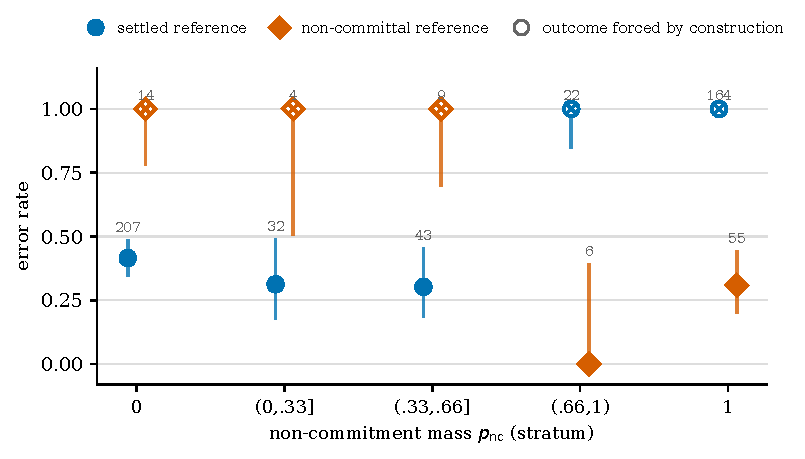
\includegraphics[width=\columnwidth]{figures/fig2_interaction.pdf}
\caption{Error rate by non-commitment stratum, split by whether the
reference answer is settled. Hollow crossed markers denote cells whose
outcome is forced by construction (answer type cannot match reference type);
filled markers are empirical. Wilson $95\%$ CIs; cell counts above each
point. The apparent interaction is largely definitional, and where it is
not, $p_{\mathrm{nc}}$ is close to uninformative.}
\label{fig:interaction}
\end{figure}

Conditional on the system taking a position, then, residual hedge mass says
little about whether that position is right. \emph{A non-commitment monitor
is a non-answer detector, not a misinformation detector}---and misinformation
is the more consequential harm.

\subsection{Failure profile is model$\times$query-type, not scale}

One might hope hedging is a small-model pathology that capability cures. It
is not. Figure~\ref{fig:regime} maps non-commitment mass over systems and
query lanes: the FT (cross-signal) lane carries the highest mass in
\emph{all five} systems. Both mid-size models commit confidently on
F---accuracy $0.55$--$0.61$, the best F-lane results we observe, exceeding the
API model---while simultaneously hedging on FT ($p_{\mathrm{nc}} = 0.73$,
$0.74$). Capability buys commitment on single-signal queries and does not buy
it where fundamentals and price action must be reconciled: precisely the
queries a user is most likely to bring to an assistant rather than to a
screener. The failure profile is therefore a property of the
model \emph{and} the query, which matters operationally---a service cannot
infer its own reliability from the model it deploys without knowing the query
mix.

\begin{figure}[t]
\centering
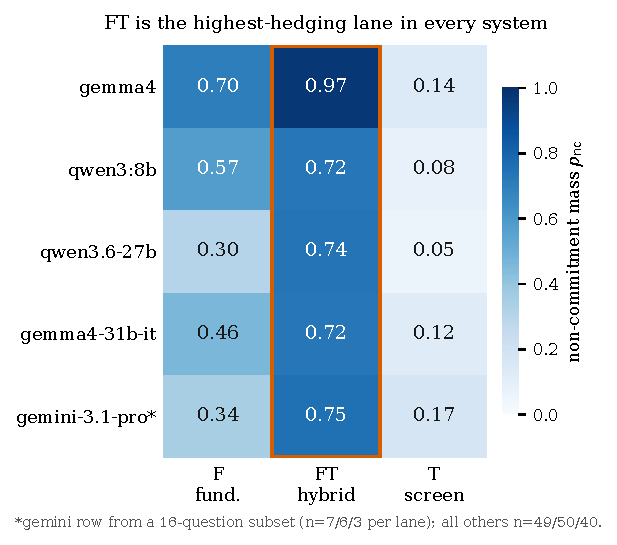
\includegraphics[width=0.86\columnwidth]{figures/fig1_regime_map.pdf}
\caption{Non-commitment mass $p_{\mathrm{nc}}$ by system and query lane
(F = fundamentals, FT = cross-signal hybrid, T = screening), final round.
Hedging concentrates on cross-signal queries in every system, independent of
scale.}
\label{fig:regime}
\end{figure}

\subsection{The uncertainty channels are not evidence-responsive}

We ran randomized, paired interventions against the stored baseline (30 F/FT
questions): removing the highest-priority \emph{present} expert indicator; a
matched placebo removing an equally-sized non-expert indicator; coherently
rewriting the trading channel to oppose the fundamental lean; and dialling
the stated horizon between three months and five years with evidence fixed.

None of the pre-registered on-target predictions is confirmed. Removing the
most important indicator produces no selective movement in any channel, and
the diagonal-versus-placebo contrast is null on every metric: the uncertainty
does not track \emph{which} evidence is present. Dialling the horizon flips
$3/30$ answers. Most informative is conflict injection: we predicted explicit
cross-signal contradiction would raise EU; instead EU \emph{falls}
($-0.041$, bootstrap CI excluding $0$) and correctness drops, because both
agents retreat to the \emph{same} non-committal answer and therefore agree
\emph{more}. \textbf{The debate looks most consensual exactly when the
evidence is most contradictory.} For an operator monitoring agreement as a
health signal, this is the worst possible failure direction.

\subsection{Agent design, not debate, drives catastrophic degradation}

Because operators configure debate panels, we ask which configuration
choices matter. On a second benchmark (37 evidence-grounded yes/no questions)
we hold benchmark, model, evidence, $K$ and schemas fixed and vary only the
second agent's role:

\begin{center}
\small
\begin{tabular}{lrrr}
\toprule
agent pair & $R_0$ acc & $R_1$ acc & rescue/loss \\
\midrule
asymmetric (skeptic)     & 0.595 & 0.351 & 1 / 10 \\
heterogeneous, symmetric & 0.595 & \textbf{0.649} & 3 / 1 \\
homogeneous (identical)  & 0.622 & 0.622 & 1 / 1 \\
\bottomrule
\end{tabular}
\end{center}

Pairing a substantive analyst with a deliberately insufficiency-hunting
skeptic is catastrophic ($\Delta$correct $-0.243$, $p{=}0.012$): the competent
analyst is pulled onto the skeptic's hedging (hedge rate $0.216 \rightarrow
0.541$, accuracy $0.622 \rightarrow 0.324$) while the skeptic barely moves.
With a symmetric partner the same analyst's hedge rate is unchanged
($0.216 \rightarrow 0.216$) and accuracy rises. Two identical analysts are
inert on every quantity ($\Delta$correct exactly $0.000$). \textbf{Role bias
does large harm; role diversity does small good; role duplication does
nothing.} A ``devil's advocate'' agent, a common design pattern, is the
specific configuration to avoid.

\subsection{Robustness of the labelling}
\label{sec:robust}

Because the taxonomy rests on classifying each reference answer as settled or
not, two independent annotators re-adjudicated all 139 from a \emph{blinded}
sheet (question, answer space, and the reference text; no schema label, no
prior classification). They agreed with each other on $86.3\%$ of commitment
calls (Cohen's $\kappa = 0.590$; Fleiss $\kappa = 0.531$ over three
annotators) and disagreed with the schema in opposite directions. Under every
annotator's labels, the majority vote, and a strict blinded consensus, hedge
collision remains modal ($0.468$--$0.670$) and the non-mechanical cell remains
at chance. Moderate $\kappa$ is honest---the judgement is genuinely
borderline at the margin---but the conclusions are invariant to it.

We also audited the reference answers themselves against the evidence packs,
since our error taxonomy inherits any defect in them. Four mechanical checks
over all 139: is an explicit superlative claim contradicted by the released
indicators; is the reference entity absent from the pack; does the reference
name more than one entity from the answer space; and does every cited figure
appear in the pack. Two references ($1.4\%$) state a superlative that the
released table falsifies---in both, the models' scored-wrong answer is the
one satisfying the reference's own stated criterion. No reference entity is
missing data. Six numeric flags are window-definition or derived-quantity
artifacts on inspection, save one (an entity whose cited leverage ratios
differ materially from the pack, though its label survives either set). We
report these rather than repair them: at $1.4\%$ they do not move any
finding, and the honest statement is that the reference set is sound on the
claims that can be checked mechanically. Judgement claims (``best
risk--reward setup'') and direction-ambiguous questions are outside what
these checks can reach.

\subsection{External validity and an open question}

\begin{figure}[t]
\centering
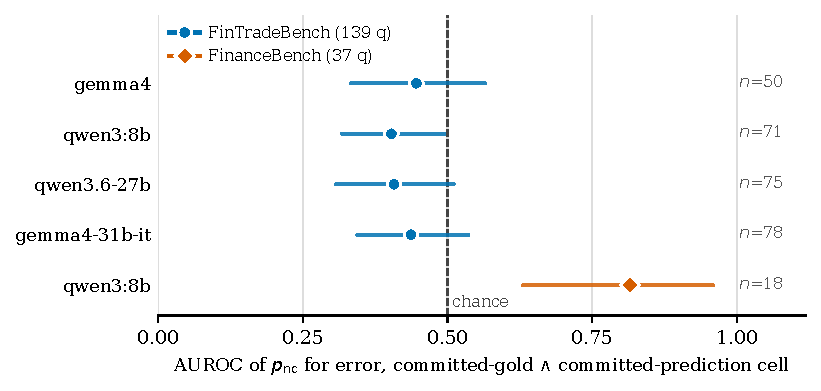
\includegraphics[width=\columnwidth]{figures/fig3_committed_cell.pdf}
\caption{Non-mechanical-cell AUROC with bootstrap $95\%$ CIs. All
FinTradeBench systems straddle chance regardless of scale, as do both
\emph{symmetric} agent configurations on the second benchmark; only the
asymmetric configuration exceeds it.}
\label{fig:boundary}
\end{figure}

The second benchmark replicates the central phenomenon more strongly---hedge
collision accounts for $79.2\%$ of errors---but its asymmetric arm initially
appeared to overturn \S5.3, giving non-mechanical-cell AUROC $0.815$
($95\%$ CI $[0.631, 0.958]$). We tested the obvious explanation, residual
hedge-mass dispersion, and it fails: within the main benchmark, across four
models and their lane-level subsets ($14$ cells), the correlation between
dispersion and non-mechanical AUROC is $\rho = -0.03$ ($p = 0.92$), with
direct counterexamples, and dispersion is collinear with the mean
($\rho = 0.96$).

The agent-design controls resolve it instead. Both \emph{symmetric}
configurations give estimates consistent with chance ($0.576$
$[0.360, 0.822]$ and $0.478$ $[0.429, 0.500]$), matching all four main-benchmark
systems; only the asymmetric arm exceeds it (Figure~\ref{fig:boundary}).
Adjacent intervals overlap, so we claim no pairwise significance---the pattern
across configurations is the evidence. We therefore report that the absence
of a misinformation signal in $p_{\mathrm{nc}}$ is not a stable property, and
that \emph{agent design, not benchmark identity}, is its identified source.

\section{Discussion: implications for operators}

\paragraph{Monitor non-commitment, not entropy.} Because non-commitment is a
discrete lexical choice, a system can be maximally self-consistent---zero
entropy, which every standard monitor scores as confident---while being
maximally uninformative. Non-commitment rate is cheap to compute from
existing outputs and directly tracks the modal failure. It is not a
replacement for accuracy evaluation: it is blind to wrong-direction
commitment, which is the more damaging harm.

\paragraph{Do not route on uncertainty.} The intuition that compute should be
spent where uncertainty is high is unsupported here: nothing in the
uncertainty profile predicts whether debate will help. Fixed-budget debate is
the defensible default until a predictive signal is demonstrated.

\paragraph{Configure panels for diversity, not adversariality.} The
devil's-advocate pattern actively degrades a competent analyst; symmetric
substantive diversity is mildly beneficial; duplication is wasted compute.

\paragraph{Score refusal as a first-class outcome.} Non-commitment is the
correct answer on a sixth of our questions. Benchmarks that score it as
failure penalise appropriate caution and reward overconfident guessing---the
opposite of what a high-stakes information service should optimise.

\section{Limitations}

Reference answers are expert-audited benchmark labels, not market outcomes;
correctness means agreement with an expert conclusion given the same
evidence. Our audit of them (\S\ref{sec:robust}) covers mechanically
checkable claims only, and $1.4\%$ fail; it cannot adjudicate judgement
claims, so the true rate of contestable references is a lower bound.
Screening-lane references are set-valued and our schema collapses them,
which is why we report T-lane wrong-direction counts as an upper bound
rather than a measurement. Commitment labelling is moderately reliable
($\kappa \approx 0.53$--$0.59$); we report invariance rather than claiming
objectivity. Pooled
rows are not independent (each question appears once per model), so per-model
results are primary and regressions cluster by ticker. EU is computed over
$N{=}2$ agents---a single edge, not a graph. The intervention suite ran on one
model at $n{=}30$ and its nulls are scoped to the hedging regime. The
second-benchmark arms are small ($n{=}37$). We audit oracle-evidence
conditions throughout; retrieval-augmented deployments add a noise source we
deliberately excluded and do not characterise.

\section{Conclusion}

Multi-agent debate makes web-facing financial assistants more stable without
making them more correct, and the standard uncertainty instrumentation cannot
tell the difference because these systems express uncertainty categorically
rather than distributionally. Their dominant failure is declining to answer
questions the evidence settles; their most damaging failure is confident
wrong entity selection, which no uncertainty channel we measured detects;
and which failure a system exhibits depends on the query type and the panel
configuration as much as on the model. We release the answer schemas,
intervention suite and per-question decompositions to support replication and
to make refusal a scoreable outcome in this setting.

\bibliographystyle{ACM-Reference-Format}
\bibliography{refs}

\end{document}
